\documentclass[aspectratio=169]{beamer}

% ── Theme ────────────────────────────────────────────────────────────
\usetheme{metropolis}
\usepackage{appendixnumberbeamer}

% ── Packages ─────────────────────────────────────────────────────────
\usepackage{booktabs}
\usepackage{pgfplots}
\pgfplotsset{compat=1.18}
\usepackage{xcolor}

% ── Colour palette (ocean) ───────────────────────────────────────────
\definecolor{deepblue}{HTML}{0A3D62}
\definecolor{midblue}{HTML}{1A6B9A}
\definecolor{accent}{HTML}{22A6DB}
\definecolor{lightblue}{HTML}{D6EAF8}
\definecolor{warncolor}{HTML}{E67E22}
\definecolor{okgreen}{HTML}{1ABC9C}

\setbeamercolor{normal text}{fg=deepblue}
\setbeamercolor{frametitle}{bg=deepblue, fg=white}
\setbeamercolor{progress bar}{fg=accent, bg=midblue!40}
\setbeamercolor{alerted text}{fg=accent}

% ── Meta ─────────────────────────────────────────────────────────────
\title{Predicting Fish Mortality}
\subtitle{in Home Aquariums}
\author{Jane Smith \\ \small CEO, Jane's Fishtank Emporium}
\date{Math 87 \quad·\quad April 2026}

% ─────────────────────────────────────────────────────────────────────
\begin{document}

% ════════════════════════════════════════════════════════════════════
\maketitle
% NOTE: One sentence of context. Don't read the title — everyone can
% see it. Just say who you are and what the talk is about.
% ════════════════════════════════════════════════════════════════════


% ════════════════════════════════════════════════════════════════════
\begin{frame}{The Problem}
% NOTE: Point at the 34% and let it land before saying anything else.
% Three bullets is plenty — resist the urge to add more.
% ════════════════════════════════════════════════════════════════════

  \begin{columns}[T]

    \begin{column}{0.38\textwidth}
      \begin{center}
        \colorbox{deepblue}{\parbox{0.9\textwidth}{%
          \vspace{0.6em}
          \begin{center}
            {\color{white}\fontsize{52}{56}\selectfont\textbf{34\%}}\\[0.4em]
            {\color{lightblue}\small of new aquariums\\
             experience a fish death\\
             in month~1}
          \end{center}
          \vspace{0.6em}
        }}
      \end{center}
    \end{column}

    \begin{column}{0.58\textwidth}
      \vspace{1.2em}
      \begin{itemize}
        \setlength{\itemsep}{1.0em}
        \item[\textcolor{warncolor}{\textbf{!}}]
              Customers blame the store
        \item[\textcolor{warncolor}{\textbf{!}}]
              Refund cost: \textasciitilde\$40 per incident
        \item[\textcolor{warncolor}{\textbf{!}}]
              No early-warning system exists
      \end{itemize}
    \end{column}

  \end{columns}

\end{frame}


% ════════════════════════════════════════════════════════════════════
\begin{frame}{Our Model}
% NOTE: Walk through the diagram left-to-right. One sentence per box.
% The footnote credits the data without cluttering the slide.
% ════════════════════════════════════════════════════════════════════

  \begin{center}
  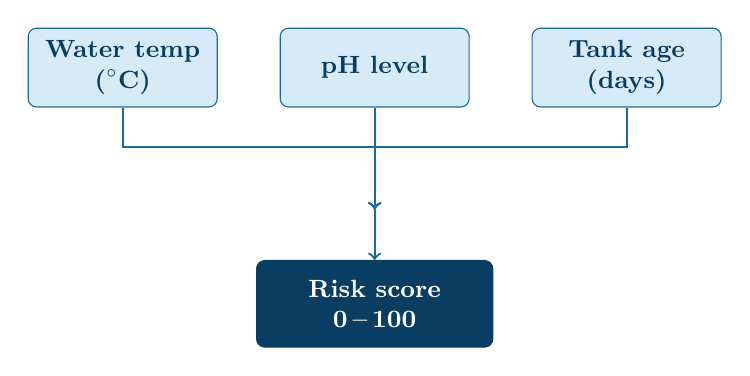
\begin{tikzpicture}[
      box/.style={draw=midblue, fill=lightblue, rounded corners=3pt,
                  minimum width=2.4cm, minimum height=1.0cm,
                  font=\small\bfseries\color{deepblue}, align=center},
      outbox/.style={draw=deepblue, fill=deepblue, rounded corners=3pt,
                     minimum width=3.0cm, minimum height=1.1cm,
                     font=\small\bfseries\color{white}, align=center},
      arr/.style={->, thick, color=midblue}
    ]
    % Input nodes
    \node[box] (temp) at (0,0)    {Water temp\\(\(^\circ\)C)};
    \node[box] (ph)   at (3.2,0)  {pH level};
    \node[box] (age)  at (6.4,0)  {Tank age\\(days)};

    % Merge point
    \coordinate (merge) at (3.2,-1.8);

    \draw[arr] (temp.south) -- ++(0,-0.5) -| (merge);
    \draw[arr] (ph.south)   -- (merge);
    \draw[arr] (age.south)  -- ++(0,-0.5) -| (merge);

    % Output node
    \node[outbox] (out) at (3.2,-3.0) {Risk score\\0\,--\,100};
    \draw[arr] (merge) -- (out.north);

  \end{tikzpicture}
  \end{center}

  \vfill
  {\footnotesize\color{gray}
   Logistic regression trained on 3 years of store data
   (\(n = 1{,}240\) tanks).}

\end{frame}


% ════════════════════════════════════════════════════════════════════
\begin{frame}{How We Built It}
% NOTE: Plain bullets are fine here — this is genuinely a list.
% Four items, each one sentence. No sub-bullets. No paragraph text.
% ════════════════════════════════════════════════════════════════════

  \begin{itemize}
    \setlength{\itemsep}{1.0em}
    \item Collected water-quality logs from 1,240 customer tanks (2021--2024)
    \item Held out 20\% of tanks as a test set before any modelling
    \item Fit a logistic regression on temperature, pH, and tank age
    \item Chose threshold score of 70 to trigger a staff follow-up call
  \end{itemize}

\end{frame}


% ════════════════════════════════════════════════════════════════════
\begin{frame}{Key Result}
% NOTE: Let the chart speak first. Then point to the two callout
% numbers on the right — those are the two things to remember.
% ════════════════════════════════════════════════════════════════════

  \begin{columns}[T]

    \begin{column}{0.60\textwidth}
      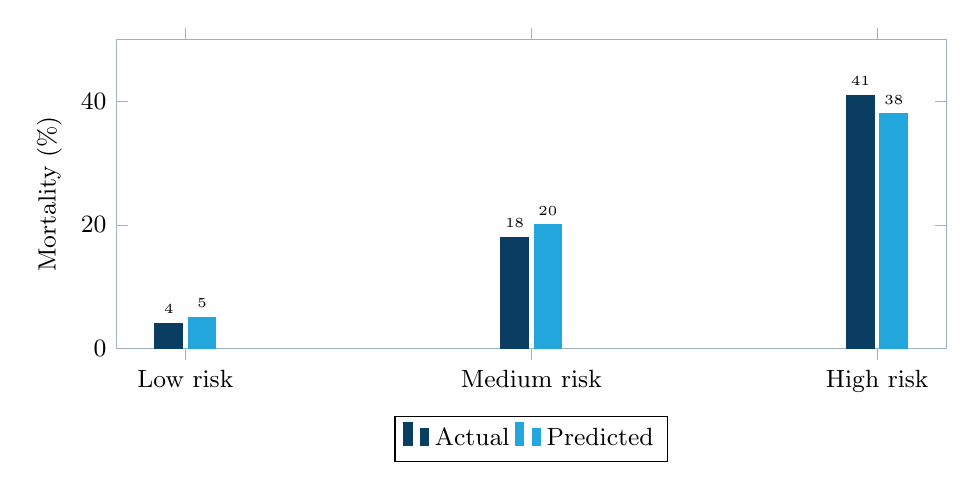
\begin{tikzpicture}
        \begin{axis}[
            ybar, bar width=10pt,
            width=\textwidth, height=5.5cm,
            symbolic x coords={Low risk, Medium risk, High risk},
            xtick=data,
            ymin=0, ymax=50,
            ylabel={\small Mortality (\%)},
            ylabel style={font=\small},
            yticklabel style={font=\small},
            xticklabel style={font=\small},
            legend style={font=\small, at={(0.5,-0.22)},
                          anchor=north, legend columns=2},
            nodes near coords,
            nodes near coords style={font=\tiny},
            axis line style={color=deepblue!40},
            tick style={color=deepblue!40},
          ]
          \addplot[fill=deepblue, draw=deepblue]
            coordinates {(Low risk,4)(Medium risk,18)(High risk,41)};
          \addplot[fill=accent, draw=accent]
            coordinates {(Low risk,5)(Medium risk,20)(High risk,38)};
          \legend{Actual, Predicted}
        \end{axis}
      \end{tikzpicture}
    \end{column}

    \begin{column}{0.36\textwidth}
      \vspace{0.6em}

      \colorbox{lightblue}{\parbox{\linewidth}{%
        \vspace{0.5em}\centering
        {\color{deepblue}\textbf{Model accuracy}}\\[0.3em]
        {\color{deepblue}\fontsize{28}{30}\selectfont\textbf{91\%}}
        \vspace{0.5em}
      }}

      \vspace{0.8em}

      \colorbox{lightblue}{\parbox{\linewidth}{%
        \vspace{0.5em}\centering
        {\color{deepblue}\small High-risk flag\\
         reduced losses \textbf{28\%}}
        \vspace{0.5em}
      }}

    \end{column}

  \end{columns}

\end{frame}


% ════════════════════════════════════════════════════════════════════
\begin{frame}{Conclusions}
% NOTE: Three cards, one sentence each. Say each one out loud with a
% single sentence of context. Then stop.
% ════════════════════════════════════════════════════════════════════

  \vspace{0.5em}
  \begin{columns}[T]

    \begin{column}{0.31\textwidth}
      \colorbox{deepblue}{\parbox{\linewidth}{%
        \vspace{1.0em}
        \begin{center}
          {\color{okgreen}\Large\(\checkmark\)}\\[0.5em]
          {\color{white}\small\textbf{Model works}}\\[0.4em]
          {\color{lightblue}\footnotesize 91\% accuracy on\\held-out test data}
        \end{center}
        \vspace{1.0em}
      }}
    \end{column}

    \begin{column}{0.31\textwidth}
      \colorbox{deepblue}{\parbox{\linewidth}{%
        \vspace{1.0em}
        \begin{center}
          {\color{okgreen}\Large\(\checkmark\)}\\[0.5em]
          {\color{white}\small\textbf{Business impact}}\\[0.4em]
          {\color{lightblue}\footnotesize 28\% fewer refund\\incidents in pilot}
        \end{center}
        \vspace{1.0em}
      }}
    \end{column}

    \begin{column}{0.31\textwidth}
      \colorbox{deepblue}{\parbox{\linewidth}{%
        \vspace{1.0em}
        \begin{center}
          {\color{accent}\Large\(\rightarrow\)}\\[0.5em]
          {\color{white}\small\textbf{Next step}}\\[0.4em]
          {\color{lightblue}\footnotesize Deploy risk-score\\alert in POS system}
        \end{center}
        \vspace{1.0em}
      }}
    \end{column}

  \end{columns}

  \vfill
  \begin{center}
    \textit{\color{gray} Thank you \quad·\quad Questions?}
  \end{center}

\end{frame}

% ════════════════════════════════════════════════════════════════════
\end{document}
